\documentclass[12pt]{standalone}
\usepackage{tikz}
\usepackage{tikz-dimline}		% Dimension (measure) lines for TikZ
\usetikzlibrary{angles, calc, decorations.pathmorphing, quotes, spy}

\begin{document}
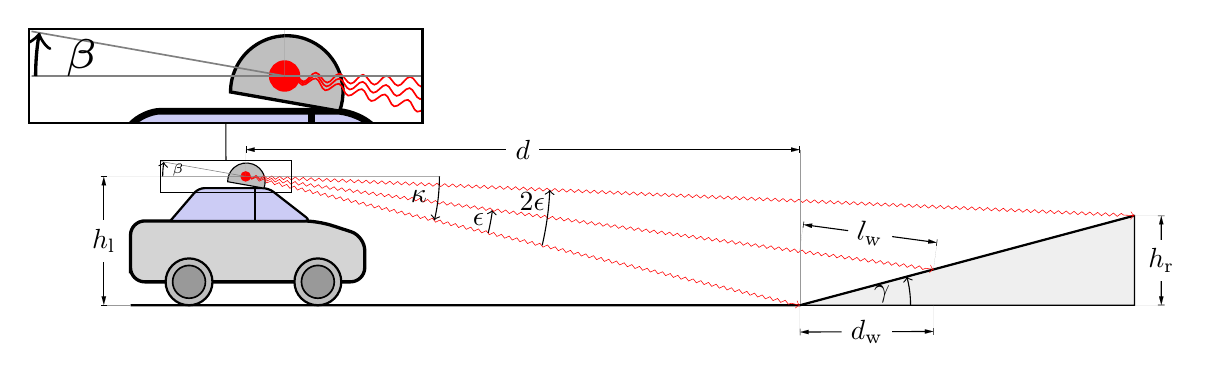
\begin{tikzpicture}[scale=0.85, spy using outlines={black, rectangle, magnification=3, width=5cm, height=1.2cm, connect spies}]
        % Define/Calc ramp parameters
        % Ramp length
        \def\rl{5};
        % Ramp angle [deg]
        \def\ra{15};
        % Ramp height
        \def\rh{{tan(\ra)*\rl}};
        % Distance of measurement line
        \def\dd{.4cm}

        % RAMP
        % Define the points
        % Left point
        \coordinate (A) at (0,0);
        % Lower right point
        \coordinate (B) at ($(A) + (\rl,0)$);
        % Upper right point
        \coordinate (C) at ($(B) + (0,\rh)$);

        % Draw and fill ramp
        \filldraw[draw=black, fill=lightgray!25] (A) -- (B) -- (C) -- cycle;
        % Draw ramp angle
        \path (A) -- (B)
        pic[draw, ->, angle radius=40pt,
                        angle eccentricity=0.75, "$\gamma$"]{angle=B--A--C};

        % Most left point at ground level
        \coordinate (D) at ($(A) + (-10,0)$);
        % Ground line
        \draw [thick] (D) -- (A) -- (C);


        % CAR
        \begin{scope}[scale=0.7]
                % Car height
                \def\ch{2}
                % Car length
                \def\cl{5}
                % Car body height
                \def\bh{\ch*0.65}
                % Roof length
                \def\rl{\cl*0.6}
                % Roof height
                \def\rh{\ch*0.35}
                % Anchor point of car body (lower left)
                \coordinate (b) at ($(D) + (0,0.5)$);
                % Offset to roof and wheels
                \coordinate (r) at ($(b) +(\cl*0.17,\ch*0.65)$);
                \coordinate (w) at ($(b) + (\cl*0.25,0)$);

                % Body
                \draw[black, fill=black!17, rounded corners=1.2ex, very thick]
                (b) -- ++(0,\bh) -- ++(\cl*1/5,0) --  ++(\cl*3/5,0) -- ++(\cl*1/5,-\bh*0.25)
                -- ++(0, -\bh*0.75) -- (b) -- cycle;
                % Roof
                \draw[very thick, rounded corners=0.5ex, fill=black!20!blue!20!white,thick]
                (r) -- ++(0.2*\rl,\rh) -- ++(0.5*\rl,0) -- ++(0.3*\rl,-\rh) -- (r);
                \draw[thick] (r)++(\rl*0.6,0) -- ++(0,\rh);

                % Wheels
                \draw[draw=black,fill=gray!50,thick] (w) circle (.5);
                \draw[draw=black,fill=gray!50,thick] (w) ++(\cl*0.55,0) circle (.5);
                % Inner wheels
                \draw[draw=black,fill=gray!80,semithick] (w) circle (.35);
                \draw[draw=black,fill=gray!80,semithick] (w) ++(\cl*0.55,0) circle (.35);

                % Lidar
                % Lidar pitch angle
                \def\lpa{10};
                \draw[black, fill=gray!50] ($(r) + (\cl*0.40,\rh)$) coordinate (le) arc(-\lpa*2:180:0.4) --cycle;

                % Car middle point
                \coordinate (m) at (\cl*0.5, \bh*0.5);
                % Lidar middle point
                \coordinate (lm) at ($(le) + (-0.39,0.25)$);
                \filldraw[red] (lm) circle(.1);
                \coordinate (idk) at ($(A)!0.4!(C)$);

                % Laser lines
                \draw[->,color=red,very thin,decorate,decoration={snake,amplitude=.2mm,segment length=1mm,post length=1mm}] (lm) -- (A)
                pic[draw, black, ->, thin, angle radius=90pt, angle eccentricity=0.95,
                                "$\epsilon$"]{angle=A--lm--idk};
                \draw[->,color=red,very thin,decorate,decoration={snake,amplitude=.2mm,segment length=1mm,post length=1mm}] (lm) -- ($(A)!0.4!(C)$);
                \draw[->,color=red,very thin,decorate,decoration={snake,amplitude=.2mm,segment length=1mm,post length=1mm}] (lm) -- ($(A)!1!(C)$)
                pic[draw, black, ->, thin, angle radius=110pt, angle eccentricity=0.95, "$2\epsilon$", pic text options={shift={(0pt,5pt)}}
                        ]{angle=A--lm--C};


                % lidar mount angle
                % Length of angle helper line
                \def\hl{4};
                \def\hll{1.8};
                \coordinate (bleb) at ($(lm) + (\hl+0.15, 0)$);
                \coordinate (blab) at ($(lm) + (\hl, -{tan{\lpa}*\hl})$);
                \coordinate (blub) at ($(lm) + (-\hll, 0)$);
                \coordinate (blob) at ($(lm) + (-\hll, +{tan{\lpa}*\hll})$);
                \draw[draw=gray, very thin] (blub) -- (lm) -- (blob)
                pic[draw, black, thin, <-, angle radius=30pt,
                                angle eccentricity=0.82, "\tiny $\beta$"]{angle=blob--lm--blub};
                \draw[draw=gray, very thin] (bleb) -- (lm);
                % pic[draw, black, thin, <-, angle radius=68pt,
                %                 angle eccentricity=0.9, "$\beta$"]{angle=blab--lm--bleb};
                \path (bleb) -- (lm) -- (A)
                pic[draw, <-, thin, angle radius=70pt,
                                angle eccentricity=0.9, "$\kappa$"]{angle=A--lm--bleb};

        \end{scope}

        % \filldraw[green] (idk) circle(.2);
        \dimline[extension start length=\dd, extension end length=\dd+1.9cm] {($(lm)+(0,\dd)$)}{($(lm -| A)+(0,\dd)$)}{$d$};
        % \dimline[extension start length=-\dd, extension end length=-\dd] {($(A)+(0,-\dd)$)}{($(B)+(0,-\dd)$)}{$l_\mathrm{r} $};
        \dimline[extension start length=-\dd, extension end length=-\dd, label style={sloped=false}] {($(B)+(\dd,0)$)}{($(C)+(\dd,0)$)}{$h_\mathrm{r}$};
        \dimline[extension start length=\dd, extension end length=\dd+1.7cm, label style={sloped=false}] {($(D)+(-\dd,0)$)}{($(lm -| D)+(-\dd,0)$)}{$h_\mathrm{l} $};

        % \dimline[extension start length=\dd, extension end length=-\dd] {($(idk)+(\dd,0)$)}{($(idk)+(\dd,-0.53)$)}{};
        % \dimline[extension start length=0, extension end length=0, label style={right, fill=none, sloped=false}] {(idk)}{($(idk)+(0,-0.53)$)}{$h_\mathrm{w}$};
        \dimline[extension start length=-\dd, extension end length=-\dd] {($(A)+(0,-\dd)$)}{($(idk)+(0,-\dd-15)$)}{$d_\mathrm{w} $};
        \dimline[extension start length=\dd, extension end length=\dd] {($(A)+(0.05,-\dd+\dd+34.3)$)}{($(idk)+(0.05,\dd)$)}{$l_\mathrm{w} $};

        % \spy[black] on ($(lm) + (-0.42, 0)$) in node at (3,4);
        \spy on ($(lm) + (-0.25, 0)$) in node at ($(lm) + (-0.3, 1.5)$);

\end{tikzpicture}
\end{document}